\chapter{Implementation}\label{chapter:impl}
Die Implementation dient der Umsetzung des im Kapitel \ref{chapter:concept} erstellten Konzepts, sodass ein Testerstellungssystem \textit{Unitcraft} zur Analyse des Hauptthemas bereitgestellt wird. Es erfolgt abschließend ein Testlauf des Programms, um die Funktionalität gewährleisten zu können. Der vollständige Quelltext ist ebenso unter \href{https://github.com/nschaefr/unitcraft}{github.com/nschaefr/unitcraft} abrufbar.

\section{Funktionalitäten}
Die im Konzept festgelegten Zielfunktionalitäten müssen mit Blick auf den Programmablaufplan [Abb. \ref{fig:pap}] zur erfolgreichen Bearbeitung der Arbeit umgesetzt werden. Dabei ist zu beachten, dass alle Funktionalitäten abgedeckt sind sowie alle Komponenten dem Konzept entsprechend zusammenarbeiten. Diese werden auf unterschiedliche Python-Dateien verteilt, um eine Struktur innerhalb des Projektes zu bewahren. Abbildung \ref{fig:dir-proj} zeigt diese Projektstruktur.\begin{figure}[h]
    \centering
    \begin{minipage}{6cm}
    \dirtree{%
    .1 unitcraft.
    .2 config.
    .3 logging\_config.py.
    .2 utils.
    .3 constants.py.
    .3 data\_handler.py.
    .3 java\_class\_extractor.py.
    .3 test\_validator.py.
    .2 llm.py.
    .2 main.py.
    }
    \end{minipage}
    \caption{Projektstruktur von \textit{Unitcraft}}
    \label{fig:dir-proj}
\end{figure}

\subsection{Nutzerabfrage}
Die Nutzerabfrage dient zur Initialisierung und ermöglicht es dem Nutzer zu Beginn des Programms die Prompt-Technik sowie die dazugehörige Temperatur festzulegen. Diese Funktionalität wird direkt in der \textit{main.py} implementiert. [Anhang \ref{lst:main}] \\Zum Erstellen einer interaktiven Befragung im Terminal ist der Import der Python-Bibliothek \textit{inquirer} notwendig. Quellcode \ref{lst:input} zeigt die Implementierung und Verwendung der Bibliothek. Dabei werden 2 Fragen als Liste von \textit{inquirer.List}-Objekten definiert. Die erste Frage stellt dem Benutzer eine Auswahl von vorher festgelegten Prompt-Techniken, die zweite von vorher definierten Temperaturwerten.\\
\lstinputlisting[caption=Interaktive Befragung in \textit{main.py} über \textit{Inquirer},captionpos=b,label={lst:input},language=python]{Assets/Code/input.py}\vspace{-.3cm}
Die Funktion \textit{inquirer.prompt(questions)} wird aufgerufen, um die erstellten Fragen dem Benutzer zu stellen und dessen Antworten in einer Variablen \textit{answers} zu speichern. Im Anschluss wird die Antwort auf die Frage der Prompt-Technik in einer Variablen \textit{prompt\_type} und die Antwort auf die Frage der Temperatur in einer Variablen \textit{temperature} gespeichert. Dies geschieht über das Initialiseren der Variablen mit dem Wert des jeweiligen Listenelements in \textit{answers}.

\subsection{Java-Datei Erfassung im Projekt}
Nach der erfolgreichen Nutzerabfrage wird in \textit{main.py} die Funtion \textit{generate\_unit\_tests} aufgerufen, welche aus \textit{llm.py} importiert ist. [Anhang \ref{lst:llm}] In dieser Funktion erfolgt das Erfassen von Java-Dateien, welche sich im \textit{src}-Verzeichnis befinden, über die Funktion \textit{find\_java\_files}. Zum Erstellen von Funktionalitäten die mit Dateien agieren, wird im Unterordner \textit{utils} eine \textit{data\_handler.py} genutzt. [Anhang \ref{lst:data}] Quellcode \ref{lst:find} zeigt die Funktion \textit{find\_java\_files} aus \textit{data\_handler.py}.\\ Zunächst wird eine leere Liste \textit{java\_files} angelegt, um die Pfade der gefundenen Java-Dateien zu speichern. Der Pfad zum Hauptverzeichnis, in dem sich die Java-Dateien befinden, wird in \textit{main\_java\_dir} initialisiert. \\
\lstinputlisting[caption=Funktion zum Erfassen der Java-Dateien in \textit{data\_handler.py},captionpos=b,label={lst:find},language=python]{Assets/Code/find_java_files.py}\vspace{-.3cm}
Dieser ist zusammengesetzt aus dem aktuellen Arbeitsverzeichnis (\textit{working\_dir}) und dem relativen Pfad \textit{src/main}. Das Arbeitsverzeichnis ist eine in \textit{data\_handler.py} definierte Variable und spiegelt das Verzeichnis wieder, in dem das Programm ausgeführt wird. Der Verzeichnisbaum wird ab \textit{main\_java\_dir} über die Funktion \textit{os.walk} rekursiv durchlaufen und jeder Pfad einer gefundenen Java-Datei zur Liste \textit{java\_files} hinzugefügt. Am Ende wird die Liste zurückgegeben. 

\subsection{Prompterstellung}
Um die durch die Nutzerabfrage initialisierten Variablen verwenden zu können, werden sie zunächst als Parameter \textit{generate\_unit\_tests} übergeben. Damit sie innerhalb \textit{llm.py} nutzbar sind, ist die Definition einer kleinen Python-Klasse sinnvoll. [Quellcode \ref{lst:config}] Damit wird ermöglicht, dass die Testparameter über ein Objekt der Klasse \textit{TestConfiguration} abrufbar sind.\\
\lstinputlisting[caption=Python-Klasse für Parameterkonfiguration in \textit{llm.py},captionpos=b,label={lst:config},language=python]{Assets/Code/testconfig.py}\vspace{-.3cm}
In Quellcode \ref{lst:generate-unit} ist zu sehen, wie ein Objekt der Klasse erstellt wird und dessen Attribute mit den Variablen der Nutzerabfrage initialisiert werden. Im Anschluss daran werden die Java-Dateien iterativ durchlaufen. Jeder Dateiinhalt wird nun über die Funktion \textit{read\_java\_file} ausgelesen, in dem \textit{open} die Datei im Lesemouds (r) öffnet und \textit{read} den gesamten Inhalt liest und zurückgibt. [Quellcode \ref{lst:read}] Dieser ist für die Erstellung des Prompts essenziell. Das \textit{config}-Objekt, der Dateipfad sowie der Inhalt der Datei werden \textit{generate\_test\_code} übergeben. [Quellcode \ref{lst:generate-unit}]\\
\lstinputlisting[caption=Funktion zum Vorbereiten der Testcoderstellung in \textit{llm.py},captionpos=b,label={lst:generate-unit},language=python]{Assets/Code/generate_unit.py}\vspace{0.5cm}
\lstinputlisting[caption=Funktion zum Auslesen des Dateiinhaltes in \textit{data\_handler.py},captionpos=b,label={lst:read},language=python]{Assets/Code/read.py}\vspace{-.3cm}
In der Funktion \textit{generate\_test\_code} findet die Prompterstellung statt. Um im Prompt relevante Informationen bereitstellen zu können, müssen bestimmte Teile des Inhalts der Java-Datei extrahiert werden. [Kapitel \ref{section:anford}]\\ Die Funktionalitäten zum Extrahieren werden in \textit{java\_class\_extractor.py} innerhalb einer Klasse \textit{JavaClassExtractor} definiert. [Anhang \ref{lst:class-extr}] In der Klasse wird über eine \textit{Regular Expression} ein \textit{Pattern} für den zu extrahierenden Inhalt erstellt, und mithilfe der \textit{re}-Funktion aus der \textit{re}-Bibliothek der Dateiinhalt auf passende Muster durchsucht. Quellcode \ref{lst:regex} zeigt die angelegten \textit{Pattern} der einzelnen Informationen.\\
\lstinputlisting[caption=\textit{RegEx-Pattern} zum Extrahieren von Inhalt in \textit{java\_class\_extractor.py},captionpos=b,label={lst:regex},language=python]{Assets/Code/reg_pattern.py}\vspace{-.3cm}
Das \textit{method\_pattern} wird zum Auffinden von Methoden genutzt und in 2 Extra-Funktionen \textit{extract\_methods\_with\_content} sowie \textit{extract\_full\_method} verwendet, um den kompletten Methodeninhalt zu extrahieren. Dabei wird in der Methode nach der ersten und letzten geschweiften Klammer gesucht und der Inhalt innerhalb dieser extrahiert und zurückgegeben. [Anhang \ref{lst:class-extr}]\\ Für jedes \textit{Pattern} existiert eine \textit{Get}-Methode, sodass die relevanten Inhalte über ein Klassenobjekt abrufbar sind. Um den Prompt final zu erstellen, ist ein Prompt-\textit{Template} notwendig, welches innerhalb \textit{constants.py} definiert ist. [Anhang \ref{lst:const}] Hier wird der in Abbildung \ref{fig:content-0} und \ref{fig:content-1} erstelle Prompt als String angelegt, welcher anhand der vom Nutzer initialisierten Variable gewählt wird. In \textit{generate\_test\_code} wird nun jede Methode iterativ durchlaufen. Dabei erfolgt die Erstellung des Prompts für die einzelne Methode, wie in Quellcode \ref{lst:prompt} erkennbar.\\ Über das \textit{Dictionary} \textit{prompt\_templates} in \textit{constants.py} wird mithilfe der Variablen für die Prompt-Technik der korrekte Prompt mit den vorher extrahierten Informationen gefüllt.\\
\lstinputlisting[caption=Prompterstellung über \textit{prompt\_templates} in \textit{llm.py},captionpos=b,label={lst:prompt},language=python]{Assets/Code/prompt.py}\vspace{-.3cm}

\subsection{API-Anfrage zur Generierung von Tests}
Die API-Anfrage und somit die Generierung des Testcodes findet in derselben Iteration statt wie die Promperstellung. Zum Durchführen einer API-Anfrage an OpenAI ist die OpenAI-Bibliothek notwendig.\\ Zusätzlich muss eine \textit{.env} angelegt werden, in der sich der \textit{OPENAI\_API\_KEY} befindet. Über die Bibiliothek \textit{load\_dotenv} kann die Funktion \textit{load\_dotenv} aufgerufen werden und somit den Inhalt von \textit{.env} nutzen. Im Anschluss daran folgt die Erstellung eines OpenAI-\textit{clients} mithilfe von \textit{OPENAI\_API\_KEY}, welcher für Anfragen an die API genutzt wird. \\Quellcode \ref{lst:api} zeigt die Anfrage in der Funktion \textit{prompt\_openai}. Hier ist zu sehen wie der \textit{client} genutzt wird, um eine Chat-Vervollständigung zu fordern. \\
\lstinputlisting[caption=API-Anfrage über OpenAI-\textit{client} in \textit{llm.py},captionpos=b,label={lst:api},language=python]{Assets/Code/prompt_openai.py}\vspace{-.3cm}
Zusätzlich werden Informationen wie \textit{model}, \textit{messages}, \textit{temperature} und \textit{max\_tokens} übergeben. Das \textit{model} wird durch den String ``gpt-4o'' festgelegt und die \textit{temperature} sowie \textit{max\_tokens} über das \textit{config}-Objekt initialisiert.\\ In der Liste \textit{messages} wird der Rolle ``System'' die in Kapitel \ref{section:prompt} definierte Systemanweisung übergeben, welche sich in \textit{constants.py} befindet. Als zweite \textit{message} mit der Rolle ``User'' wird der im vorherigen Kapitel erstellte Prompt bereitgestellt. Die generierte Antwort des Modells wird nun aus der API-Antwort extrahiert in dem wir \textit{choices[0]} und deren Inhalt \textit{message.content} in der Variablen \textit{test\_code} speichern.\\ Da das Sprachmodell aufgrund der 
Systemanweisung nur Code zurückgibt und dieser in den meisten Fällen im \textit{markdown}-Codeformat formatiert ist, übergeben wir \textit{test\_code} einer Funktion \textit{remove\_format}, welche über ein \textit{Pattern} die Zeichen ``\`{}\`{}\`{}'' sucht und über die \textit{strip}-Funktion entfernt. [Quellcode \ref{lst:strip}]\\
\lstinputlisting[caption=Entfernen des \textit{markdown}-Codeformats im \textit{test\_code} in \textit{llm.py},captionpos=b,label={lst:strip},language=python]{Assets/Code/strip.py}\vspace{-.3cm}

\subsection{Testüberprüfung mit Repair Rounds}
Im Anschluss an die Testgenerierung erfolgt die Überprüfung der Kompilierbarkeit des vom Sprachmodell erstellten Testcodes. Hierbei wird vorausgesetzt, dass der Inhalt in eine \textit{test file} geschrieben wird. In \textit{data\_handler.py} befindet sich die Funktion \textit{create\_test\_file}, die eine solche Funktionalität abdeckt. [Quellcode \ref{lst:create_file}]\\
Zunächst wird der Pfad der \textit{test file} aus einer Kombination des \textit{test file} Verzeichnisses und dem relativen Pfad der \textit{java file} erstellt. Mithilfe von \textit{with open()} wird eine Datei im Schreibmodus geöffnet und über die \textit{write} Funktion eine Zeichenkette, in unserem Falle der generierte Testcode, in die geöffnete Datei geschrieben. \\Die Funktion \textit{create\_test\_file} gibt den erstellten Pfad zurück, sodass im Anschluss mit ihm gearbeitet werden kann.\\[0.4cm] 
\lstinputlisting[caption=Erstellen einer \textit{test file} mit generiertem Inhalt in \textit{data\_handler.py},captionpos=b,label={lst:create_file},language=python]{Assets/Code/create_test_file.py}\vspace{-.3cm}
Der Pfad findet nun Verwendung innerhalb \textit{validate\_test} in \textit{test\_validator.py}. [Anhang \ref{lst:valid}] Neben der Extrahierung der Testanzahl zur Ausgabe in der Konsole, sowie der Initialisierung des \textit{file names}, wird eine Funktion \textit{run\_maven\_test} aufgerufen, welche die Kompilierbarkeit überprüft. [Quellcode \ref{lst:test_valid}] \\Innerhalb dieser Funktion wird der Import \textit{subprocess} benötigt, um externe Prozesse ausführen und dessen Ausgabe erfassen zu können. \\
\lstinputlisting[caption=Validieren der Kompilierbarkeit des Tests in \textit{test\_validator.py},captionpos=b,label={lst:test_valid},language=python]{Assets/Code/validate_test.py}\vspace{-.3cm}
Quellcode \ref{lst:run_maven} zeigt die Implementation von \textit{run\_maven\_test}. Über \textit{subprocess.run()} wird ein \textit{maven}-Befehl zum Testkompilieren in einem neuen Prozess ausgeführt und dessen Ausgabe abgefangen.
Mithilfe des Setzens von \textit{capture\_output} und \textit{text} auf \textit{True} kann die Ausgabe als Zeichenkette zurückgegeben werden. Ist diese erfolgreich (\textit{Returncode 0}) wird \textit{True, None} zurückgegeben um anzuzeigen, dass der Test erfolgreich war und keine Fehler beim Kompilieren aufgetreten sind.\\
\lstinputlisting[caption=Ausführen des \textit{mvn}-Befehls zum Testkompilieren in \textit{test\_validator.py},captionpos=b,label={lst:run_maven},language=python]{Assets/Code/run_maven.py}\vspace{-.3cm} 
Im anderen Falle wird der Error mit einem \textit{False} zurückgegeben und sorgt dafür, dass innerhalb \textit{validate\_test} die Funktion \textit{handle\_error} zur Bearbeitung des Errors aufgerufen wird. Neben der Übergabe des \textit{Errors} wird eine Variable \textit{attempt} als Parameter übergeben, sodass nach 2 \textit{Repair Rounds} eine Aufforderung zum Löschen des fehlerverursachenden Codes oder im Anschluss daran die Aufforderung zum Löschen der gesamten \textit{test file} realisiert werden kann. \\Quellcode \ref{lst:repair} zeigt den ausgeführten Code innerhalb der ersten beiden \textit{Repair Rounds}.\\
\lstinputlisting[caption=Durchführung der \textit{Repair Rounds} in \textit{test\_validator.py},captionpos=b,label={lst:repair},language=python]{Assets/Code/repair_round.py}\vspace{-.3cm}
Somit wird der in \textit{constants.py} definierte Prompt zum Reparieren des Codes genutzt, in dem er mit dem spezifischen \textit{Error} sowie dem Testinhalt gefüllt wird. Mithilfe des Imports von \textit{prompt\_openai} kann ein erneuter Prompt an das Sprachmodell gestellt werden. Die \textit{response} wird in einer Variablen \textit{corr\_class} abgespeichert und der Inhalt der \textit{test file} dementsprechend aktualisiert. Die aktualisierte Datei wird nun wieder auf Kompilierbarkeit überprüft. \\Ist die Anzahl der \textit{Repair Rounds} ausgeschöpft, so wird beim dritten Versuch der Prompt zum Löschen des fehlerverursachenden Codes aufgerufen sowie im letzten Versuch die Datei gelöscht. [Quellcode \ref{lst:delete}]\\
\lstinputlisting[caption=Löschen von Code bzw. der Testdatei in \textit{test\_validator.py},captionpos=b,label={lst:delete},language=python]{Assets/Code/delete_round.py}\vspace{-.3cm}
Durch die oben beschriebene und in \textit{data\_handler.py} implementierte Funktion \textit{create\_test\_file} wird ein erfolgreiches Ablegen der \textit{test file} im korrekten Pfad gewährleistet. Während der Überprüfung auf Kompilierbarkeit aktualisiert sich lediglich der Inhalt und der Pfad wird dementsprechend beibehalten.

\subsection{Logging}
Wie zu Beginn in Abbildung \ref{fig:dir-proj} zu erkennen, befindet sich im \textit{config}-Verzeichnis eine \textit{logging\_config.py}. [Anhang \ref{lst:log}] Diese richtet eine benutzerdefinierte Logger-Konfiguration ein, welche farbige und formatierte Log-Nachrichten ausgibt. Somit werden Log-Nachrichten besser lesbar und leichter unterscheidbar, insbesondere in einer Konsole.\\ Dazu werden vorerst Farb- und Formatidefinitionen mithilfe von \textit{ANSI-Escape-Codes} definiert. \textit{SUCCESS} setzt die Textfarbe auf Grün, \textit{FAIL} auf Rot, \textit{BOLD} setzt den Text auf fett und \textit{RESET} setzt alle Textformatierungen zurück. [Quellcode \ref{lst:color}]\\
\lstinputlisting[caption=Farb- und Formatdefinitionen in \textit{logging\_config.py},captionpos=b,label={lst:color},language=python]{Assets/Code/color.py}\vspace{-.3cm}
Die Nutzung von \textit{logging} ermöglicht das Konfigurieren eines Logging-Systems, um die eben gezeigten Formatierungen zu verwenden. Quellcode \ref{lst:setup} zeigt die Funktion \textit{setup\_logging}, welche zum Einrichten des \textit{Loggers} dient. \\
\lstinputlisting[caption=Funktion zum Einrichten des Loggers in \textit{logging\_config.py},captionpos=b,label={lst:setup},language=python]{Assets/Code/setup_logging.py}\vspace{-.3cm}Hierbei wird die Standard-Log-Ebene auf \textit{INFO} gesetzt und ein \textit{Stream-Handler} erstellt, der die Log-Nachrichten an die Konsole ausgibt.
Über die Funktion \textit{setFormatter} wird ein benutzerdefinierter Formatter für den Stream-Handler festgelegt. Dieser ist in Form einer Klasse in Quellcode \ref{lst:formatter} implementiert.\\
\lstinputlisting[caption=Benutzerdefinierte Formatter-Klasse in \textit{logging\_config.py},captionpos=b,label={lst:formatter},language=python]{Assets/Code/custom_formatter.py}\vspace{-.3cm}
\textit{FORMATS} definiert das Format für jede Log-Ebene:
\begin{itemize}
    \setlength{\parskip}{1pt}
    \item logging.DEBUG: Normale Schrift, keine besondere Farbe
    \item logging.INFO: Normale Schrift, keine besondere Farbe
    \item logging.WARNING: Fett gedruckter Text
    \item logging.ERROR: Roter Text
    \item logging.CRITICAL: Roter und fett gedruckter Text
\end{itemize}
Die in Quellcode \ref{lst:format} implementierte Methode \textit{format} überschreibt die \textit{format}-Methode der Basisklasse, was ermöglicht, dass die Log-Nachricht ``\textit{TEST COMPILATION SUCCESSFUL}'' grün erscheint. Durch das Erstellen eines Formatter-Objekts mit dem gewählten Format, wird die Nachricht formatiert zurückgegeben.\\
\lstinputlisting[caption=Spezifisches Format für SUCCESS-Ausgabe in \textit{logging\_config.py},captionpos=b,label={lst:format},language=python]{Assets/Code/format.py}\vspace{-.3cm}

\section{Integration von SonarQube, Plugins, Dependencies}\label{sec:sonar}
Damit dem Sprachmodell die Verwendung von Frameworks ermöglicht wird, müssen diese in Form von \textit{Dependencies} in das zu testende Java-Projekt innerhalb der \textit{pom.xml} integriert werden. [Anhang \ref{lst:pom}] Benötigt wird das Framework \textit{Mockito} sowie \textit{JUnit-Jupiter}.\\
Somit hat das Sprachmodell umfangreiche Möglichkeiten um Tests zu generieren. Zusätzlich dazu ist das \textit{JaCoCo}-Plugin essenziell, um eine \textit{Coverage} zu erzeugen, welche von \textit{SonarQube} ausgewertet wird. [Anhang \ref{lst:pom}]
\\Zur Verwendung von SonarQube als \textit{Coverage}-Analyse Framework gibt es verschiedene Möglichkeiten. Eine gängige Methode ist das Installieren einer lokalen Instanz via \textit{Docker}. \cite*{TryOutSonarQube} Hierbei lässt sich der Server über einen simplen Docker-Befehl starten:\\[-.2cm]
\lstinputlisting[caption=\textit{Docker}-Befehl zum Starten der \textit{SonarQube}-Instanz, captionpos=b,label={lst:docker},language=bash,numbers=none]{Assets/Code/docker.sh}\vspace{-.3cm} Die Instanz ist nun über \textit{http://localhost:9000} erreichbar und es besteht die Möglichkeit sich als System Administrator (Login: admin, Passwort: admin) einzuloggen.\\ Nach dem Erstellen eines neuen Projektes in \textit{SonarQube} nutzt man folgendem \textit{Template}-Befehl, um eine Codeanalyse zu starten:\\[-.2cm]
\lstinputlisting[caption=\textit{Template}-Befehl zum Starten der Codeanalyse mit \textit{SonarQube}, captionpos=b,label={lst:sonar},language=bash,numbers=none]{Assets/Code/sonar.sh}\vspace{-.3cm}
Bei einem erfolgreichem Ausführen der Analyse sind die generierten Metriken über das \textit{User Interface} der \textit{SonarQube}-Instanz zu finden

\section{Testdurchlauf}
Um eine erfolgreiche Implementierung abschließen zu können, ist ein Testdurchlauf essenziell, sodass alle Funktionalitäten getestet werden.\\ Als Testprojekt wird ein einfacher Rechner genutzt, welcher die Addition und Subtraktion zweier Zahlen berechnet. In Abbildung \ref{fig:dir-proj-test} ist die Struktur des Projektes dargestellt.\begin{figure}[h]
    \centering
    \begin{minipage}{8cm}
        \dirtree{%
        .1 calculator-maven-project.
        .2 pom.xml.
        .2 src.
        .3 main.
        .4 java.
        .5 com.
        .6 example.
        .7 calculator.
        .8 Calculator.java.
        .3 test.
        }        
    \end{minipage}
    \caption{Projektstruktur des Testprojektes}
    \label{fig:dir-proj-test}
\end{figure}\\
Quellcode \ref{lst:calc} zeigt \textit{Calculator.java} und somit die Programmlogik des Rechners.\\
Nach erfolgter Integration von \textit{Dependencies}, \textit{Plugins} sowie \textit{SonarQube} (beschrieben in Kapitel \ref{sec:sonar}) muss ein Ziel definiert werden, um den Testdurchlauf als erfolgreich eingliedern zu können. \\
\lstinputlisting[caption=Programmlogik des Rechners in \textit{Calculator.java},captionpos=b,label={lst:calc},language=java]{Assets/Code/calculator.java}\vspace{-.3cm}
Dabei liegt der Fokus auf folgenden Aspekten:
\begin{itemize}
    \setlength{\parskip}{1pt}
    \item Erfolgreiche Nutzerabfrage
    \item Erstellen der Tests und korrektes Ablegen im richtigen Pfad
    \item Korrekte Darstellung der \textit{Logs}
    \item Erfassen der Metriken mit \textit{SonarQube}
\end{itemize}
In unserem Falle lautet der Pfad ``\textit{src/test/java/com/example/calculator/CalculatorTest.java}''.
Beim Ausführen von \textit{python3 path/to/main.py} im Verzeichnis \textit{calculator-maven-project} erscheint die in Abbildung \ref{fig:user} dargestellte Ausgabe.\begin{figure}[h]
    \centering
    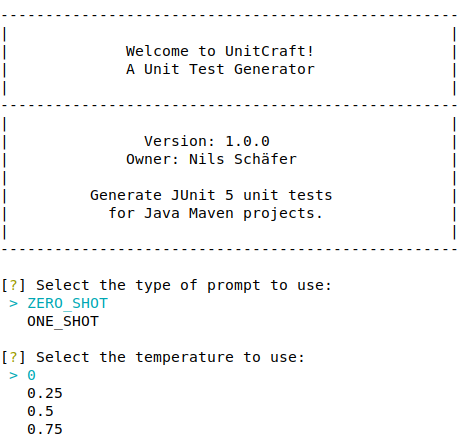
\includegraphics[width=0.48\textwidth]{Assets/Images/user.png}
    \caption{Ausgabe der Nutzerabfrage in \textit{unitcraft}}
    \label{fig:user}
\end{figure}
\\
Zu sehen ist eine Auswahl an Prompt-Techniken sowie Temperaturwerten, die der Nutzer wählen kann.
Nach Auswahl der relevanten Parameter erfolgt die Erstellung der Tests. Abbildung \ref{fig:tests} zeigt die Ausgabe in der Konsole, in der ebenso erkennbar ist, dass das \textit{logging} funktioniert. \\Es wurden zwei Java-Dateien mit jeweils 6 bzw. 5 Tests erstellt. [Anhang \ref{lst:test-1} + \ref{lst:test-2}] Die erste Datei deckt die Methode der Addition und die zweite die der Subtraktion ab. Beide Testdateien sind beim ersten Versuch erfolgreich kompiliert. Der komplette Prozess dauerte 22 Sekunden.\begin{figure}[h]
    \centering
    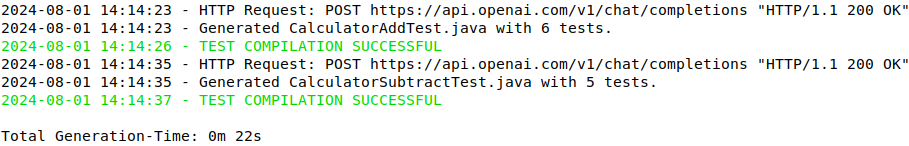
\includegraphics[width=1\textwidth]{Assets/Images/tests.png}
    \caption{Ausgabe der Logs für die erstellten Tests in \textit{unitcraft}}
    \label{fig:tests}
\end{figure}
\\
Der oben genannte Pfad für die Testdateien wurde korrekt angelegt, sowie die Dateien selbst in diesem abgelegt. [Abb. \ref{fig:path}]\begin{figure}[h]
    \centering
    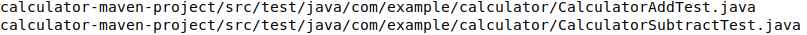
\includegraphics[width=1\textwidth]{Assets/Images/path.png}
    \caption{Ausgabe des Pfades für die erstellten Testdateien}
    \label{fig:path}
\end{figure}
\\
Wenden wir das in Kapitel \ref{sec:sonar} beschriebene Vorgehen zum Erzeugen der Testmetriken mit \textit{SonarQube} an, erkennen wir eine \textit{Line-} sowie \textit{Branch Coverage} von 100\%, was einer \textit{Overall Coverage} von 100\% entspricht. Ebenso erreichen wir eine Erfolgsquote von 100\%, was bedeutet, dass kein Test während der Laufzeit fehlgeschlagen ist oder aufgrund von falscher Programmlogik einen Fehler wirft.\\\\
Abschließend kann man sagen, dass der Testdurchlauf sowie die zugrundeliegende Implementation erfolgreich ist, und eine solide Basis für die in Kapitel \ref{chap:analysis} stattfindende Analyse schafft.




